%-----------------------------------------------------------------------------%
\chapter{LANDASAN TEORI}
Pada bab ini akan dijelaskan mengenai teori dasar dan metode yang digunakan pada penelitian ini. 
%-----------------------------------------------------------------------------%

%
\vspace{4.5pt}

\section{Tinjauan Pustaka}
Pada bagian ini akan dijelaskan teori-teori terkait yang akan digunakan dalam aplikasi klasifikasi teks 
\subsection{Pemrosesan Bahasa Alami}
Pemrosesan Bahasa Alami atau \textit{Natural Language Processing} (NLP) adalah 
bidang penelitian dan aplikasi yang mengeksplorasi bagaimana komputer 
dapat digunakan untuk memahami dan memanipulasi teks atau pidato bahasa 
alami. Penelitian NLP bertujuan untuk mengumpulkan pengetahuan tentang 
bagaimana manusia memahami dan menggunakan bahasa sehingga alat dan 
teknik yang tepat dapat dikembangkan untuk membuat sistem komputer 
memahami dan memanipulasi bahasa alami untuk melakukan tugas yang 
diinginkan. Dasar-dasar NLP terletak pada sejumlah ilmu, seperti ilmu 
komputer dan informasi, linguistik, matematika, teknik elektro dan 
elektronika, kecerdasan buatan dan robotika, dan psikologi. Aplikasi NLP 
mencakup sejumlah bidang studi, seperti terjemahan mesin, pemrosesan 
teks bahasa alami dan \textit{summarization}, antarmuka pengguna, 
pencarian informasi multibahasa dan lintas bahasa (CLIR), pengenalan 
ucapan, kecerdasan buatan, dan sistem pakar. Di bawah ini terdapat 7 
tingkatan \textit{interdependent} yang digunakan untuk mengekstrak 
makna dari teks atau bahasa lisan \cite{9}:
\begin{enumerate}[leftmargin=*]
	\item \textit{Phonetic} atau \textit{phonological level} adalah 
	tingkatan yang berurusan dengan pengucapan.
	\item \textit{Morphological level} adalah tingkatan yang berhubungan 
	dengan makna kata, awalan kata dan akhiran kata.
	\item \textit{Lexical Level} adalah tingkatan yang berhubungan dengan 
	leksikal kata dan \textit{Part Of Speech}
	\item \textit{Syntactic level} adalah tingkatan yang berhubungan 
	dengan tata Bahasa dan struktur kalimat.
	\item \textit{Semantic Level} adalah tingkatan yang berhubungan dengan 
	makna kata dan kalimat.
	\item \textit{Discourse Level} adalah tingkatan yang berhubungan 
	dengan struktur berbagai jenis teks menggunakan struktur dokumen.
	\item \textit{Pragmatic Level} adalah tingkatan yang berhubungan 
	dengan pengetahuan dari luar pada isi sebuah dokumen.
\end{enumerate}

\subsection{Analisis Sentimen}
Analisis sentimen atau biasa disebut \textit{opinion mining} adalah 
bidang studi yang menganalisis opini, sentimen, evaluasi, penilaian, 
sikap, dan emosi orang-orang terhadap entitas seperti produk, layanan, 
organisasi, individu, isu, peristiwa, topik, dan atribut mereka. Ada 
juga istilah yang lain dengan tugas yang tidak jauh berbeda, misalnya 
analisis sentimen, \textit{opinion mining}, \textit{opinion extraction}, \textit{sentiment} \textit{mining}, \textit{subjectivity analysis}, \textit{affect analysis}, \textit{emoticon analysis}, \textit{review mining}, dan sebagainya. Istilah tersebut merupakan bagian dari analisis sentimen atau \textit{opinion mining}. Istilah analisis sentimen pertama kali muncul di Nasukawa dan Yi (2003), dan istilah \textit{opinion mining }pertama kali muncul di Dave et al. (2003). Namun, penelitian tentang sentimen dan pendapat muncul lebih awal (Das and Chen, 2001; Morinaga et al., 2002; Pang et al., 2002; Tong, 2001; Turney, 2002; Wiebe, 2000). Analisis sentimen atau \textit{opinion mining }berfokus pada opini yang mengungkapkan atau menyiratkan sentimen positif atau negatif \cite{10}.
\subsection{Pembelajaran Mesin}
Tujuan utama Pembelajaran Mesin adalah untuk memodelkan hubungan antara 
masukan dan keluaran. Pembelajaran mesin menyediakan teknik yang secara 
otomatis dapat membangun model komputasi dari hubungan kompleks dengan 
memproses data yang ada dan memaksimalkan kriteria kinerja yang 
bergantung pada masalah. Proses otomatis pembuatan model disebut 
\textit{training} dan data yang digunakan untuk tujuan pelatihan 
disebut data \textit{training}.\textit{ }Model yang sudah dilatih 
dapat memberikan informasi baru tentang bagaimana variabel masukan 
dipetakan ke keluaran dan dapat digunakan untuk membuat prediksi untuk 
nilai masukan baru yang bukan merupakan bagian dari data \textit{training}. Untuk dapat mempelajari model yang akurat, algoritme pembelajaran mesin membutuhkan sejumlah besar data \textit{training}. Oleh karena itu, langkah pertama yang penting dalam menggunakan teknik pembelajaran mesin adalah mengumpulkan sekumpulan contoh data \textit{training }dan menyimpannya dalam bentuk yang sesuai untuk keperluan komputasi.

Pembelajaran mesin dapat dilakukan di banyak domain seperti diagnosis 
medis, bioinformatika, informatika kimia, analisis jaringan sosial, 
analisis pasar saham, dan robotika. Kinerja model pembelajaran mesin 
bergantung pada banyak faktor seperti jumlah dan kualitas data 
pelatihan, kompleksitas dan bentuk hubungan antara variabel masukan dan 
keluaran, dan kendala komputasi seperti waktu pelatihan dan memori yang 
tersedia \cite{11}.

\subsection{Text Preprocessing}
\textit{Text} \textit{Preprocessing} bertujuan untuk meminimalisir 
kata yang akan digunakan dalam teks. Pada media sosial Indonesia seperti 
Twitter atau Facebook, pengguna sering menggunakan bahasa non-formal 
dibanding formal seperti mengganti kata dengan angka, mengulangi huruf 
yang sama, dan menggunakan kata non-formal untuk menggantikan kata 
formal \cite{5}. Untuk memproses kata-kata seperti itu, maka akan 
dilakukan beberapa teknik \textit{text} \textit{preprocessing }
sebagai berikut: 
\subsubsection{\textit{Case Folding}}
\textit{Case Folding }adalah tahap mengubah teks menjadi huruf kecil. 
Huruf-huruf yang ditangani dimulai dari a-z.
\subsubsection{\textit{Remove Hashtag}, URL, \textit{Mention}}
\textit{Remove Hashtag, }URL\textit{, Mention }adalah tahap 
menghapus semua \textit{hashtag}, URL, dan \textit{mention }yang 
terdapat pada teks. Contoh "@andi filmnya bagus https://... \#bagus", 
maka akan menjadi "filmnya bagus".
\subsubsection{\textit{Remove Punctuation}}
\textit{Remove Punctuation }adalah tahap menghapus tanda baca yang 
terdapat pada teks. Tanda petik ("), tanda petik tunggal ('), tanda 
seru (!), tanda tanya (?) dan tanda pemisah (-) akan menjadi 
pengecualian pada \textit{preprocessing }ini, karena akan digunakan 
sebagai fitur \textit{punctuation based}. Contoh tanda baca yang akan 
dihapus adalah "\%", "\&", "*", "\{\}", "()", "[]", ":", dan lain-lain.
\subsubsection{\textit{Tokenization}}
\textit{Tokenization} adalah tahap memecahkan kalimat menjadi 
token-token. Tiap token yang dihasilkan tidak harus terdiri dari satu 
kata. Satu token bisa saja menghasilkan dua kata. 
\subsubsection{\textit{Misuse of Word}}
Setelah tahap \textit{tokenization}, tahap selanjutnya adalah 
mengubah penyalahgunaan kata, sebagai contoh: "ASIIIKKK", terdapat 
penyalahgunaan huruf yaitu "I" dan "K". Sehingga akan diubah menjadi 
"ASIK". Setiap kata yang terdapat huruf sama dan bersebelahan akan 
dijadikan menjadi 1 huruf, meskipun kata tersebut menjadi kata yang 
tidak memiliki makna, contohnya kata "tanggung", kata tersebut akan 
diubah menjadi "tangung" sehingga menjadi tidak memiliki makna. Hal 
ini tidak masalah untuk dilakukan, karena pada penelitian ini tidak 
dilakukan pada \textit{semantic level} atau tidak mementingkan makna 
dari sebuah kata.  
\subsubsection{\textit{Abbreviation Word}}
Setelah tahap \textit{misuse of word, }tahap selanjutnya adalah 
mengubah kata-kata yang menggunakan singkatan. Sebagai contoh: "km" 
menjadi kamu.
\subsubsection{\textit{Stopword Removal}}
Setelah tahap \textit{abbreviation word}, maka teks akan siap 
memasuki tahap berikutnya yaitu \textit{stopword removal}. Pada tahap 
ini kata-kata yang terdapat pada daftar \textit{stopword }akan 
dihilangkan dari teks\textit{. Stopword }adalah kata-kata yang 
dianggap tidak memberi pengaruh terhadap teks. Sebagai contoh, kata 
"yang", "dan", "di", "ke", dan "dari". Masih terdapat banyak 
lagi kata-kata yang termasuk dalam \textit{stopword }ini.
\subsubsection{\textit{Stemming}}
Setelah tahap \textit{stopword removal}, maka teks akan siap memasuki 
tahap berikutnya yaitu \textit{stemming. }Pada tahap ini token-token 
pada teks akan diubah menjadi kata dasar. Fitur ini akan menggunakan 
\textit{library} python yaitu \textit{stemmer }Sastrawi. Pada tahap 
ini penulis akan menggunakan library yang terdapat pada python untuk 
melakukan \textit{stemming}. \textit{Stemming} yang digunakan 
adalah algoritme Nazief dan Adriani. \textit{Stemming }ini biasanya 
bertujuan untuk menghapus \textit{suffixes}, dan sering digunakan 
pada \textit{text search},\textit{ machine translation},\textit{ 
	document summarization},\textit{ text classification}. \textit{
	Affixes }dapat dibagi menjadi dua, yaitu \textit{inflectional }atau 
\textit{derivational}. Contoh pada kata kerja \textit{English}, 
"\textit{teach}" dapat ditambah dengan \textit{inflectional 
	suffixes }"-\textit{es}" sehingga menjadi kata kerja tunggal "\textit{teaches}". Selain itu kata "\textit{teach}" juga dapat 
ditambah dengan \textit{derivational suffixes }"-\textit{er}" 
sehingga menjadi kata benda "\textit{teacher}". Dalam Indonesia, 
\textit{inflectional suffixes }hanya terdapat pada \textit{suffixes}
, sedangkan \textit{derivational suffixes} terdapat pada \textit{
	prefix}, \textit{suffixes} atau gabungan keduanya \cite{12}.

Dalam Indonesia, terdapat dua macam \textit{inflectional suffixes} [Moeliono dan Dardjowidjojo 1988]:
\begin{enumerate}[leftmargin=*]
	\item \textit{Particle} (P) {“-kah”, ”-lah”, ”-tah”, “-pun”}\\
	\textit{Particle }di atas adalah imbuhan yang tidak akan mengubah kata 
	menjadi kata kerja atau kata benda. Contoh, \textit{suffix }"-lah" 
	ketika ditambahkan pada kata "duduk" akan menjadi "duduklah".
	\item \textit{Possessive Pronouns} (PP) {“-ku”, “-mu”, “-nya”}\\
	\textit{Possessive Pronouns }akan mengubah kata menjadi hubungan 
	kepemilikan. Contoh, \textit{suffix} "-nya" ketika ditambahkan pada 
	kata "buku" akan menjadi "bukunya".
\end{enumerate}

\textit{Derivational Prefixes }(DP) \{"be-," "di-," "ke-," 
"me-," "pe-," "se-," and "te-"\}. \textit{Prefix }"me-" dapat muncul sebagai "me-", "mem-", " meng-", "men-", dan "meny-" bergantung dengan kata dasarnya. Sebagai contoh, \textit{derivational prefixes} "se-", "peng-", "ke-" ditambahkan pada kata "tahu" dan dengan \textit{suffixes }"-an", "-ku" akan menghasilkan kata "sepengetahuanku" \cite{12}.

\textit{Derivational Suffixes} (DS)\textit{ }\{"-i", "-kan", 
"-an"\} hanya boleh digunakan satu \textit{suffixes} saja pada kata 
dasar. Sebagai contoh, kata "lapor" ditambahkan dengan \textit{suffix
} "-kan" menghasilkan "laporkan" \cite{12}.

\textit{Derivational Confix (DC) }\{"be-an", "me-i", "me-kan", 
"di-i", "dikan"\} adalah gabungan dari \textit{prefix }dan
\textit{ suffix}. Sebagai contoh, \textit{prefix }"ke-" dan 
\textit{suffix }"-an" ditambahkan pada kata dasar "dalam" 
menghasilkan "kedalaman". Berikut adalah contoh \textit{affix }model 
yang mungkin terbentuk pada kata dasar:

\begin{table}[H]
	\small
	\begin{adjustbox}{width=1\textwidth}
	\begin{tabular}{|>{\centering\arraybackslash}p{13.55cm}|}
		\hline
		[ [ DP +][ DP +] DP +] kata dasar [ [+DS ][+PP ][+P ] ]\\
		\hline
	\end{tabular}
	\end{adjustbox}
\end{table}
\vspace{-0.5cm}
\noindent Berikut merupakan langkah dan proses yang dilakukan dalam \textit{stemming} [12]:
\begin{enumerate}[leftmargin=*]
	\item Menghapus semua \textit{inflectional suffixes }pada kata 
	masukan. Proses \textit{stemming }berhenti, jika kata masukan\textit{ 
	}terdapat pada kamus kata dasar. Jika tidak, maka berdasarkan \textit{
	affix }model, yang tersisa adalah \textit{derivational suffixes}. Berikut adalah model yang mungkin terbentuk:
	\begin{table}[H]
		\hspace{12pt}
		\centering
		\small
		\begin{adjustbox}{width=1\linewidth}
			\begin{tabular}{|>{\centering\arraybackslash}p{\linewidth}|}
				\hline
				[ [ DP +][ DP +] DP +] kata dasar [+DS ]\\
				\hline
			\end{tabular}
		\end{adjustbox}
	
		\hspace{12pt}
	\end{table}
	\item Menghapus semua \textit{derivational suffixes}. Berikut model yang terbentuk:
	\begin{table}[H]
		\hspace{12pt}
		\centering	
		\small
		\begin{adjustbox}{width=1\linewidth}
		\begin{tabular}{|>{\centering\arraybackslash}p{\linewidth}|}
			\hline
			[ [ DP +][ DP +] DP +] kata dasar\\
			\hline
		\end{tabular}
		\end{adjustbox}
		\hspace{12pt}
	\end{table}
	\vspace{-0.7cm}
	\item Menghapus semua \textit{derivational prefixes}.
	\begin{enumerate}[label={\arabic*},leftmargin=*]
		\item Syarat proses stemming berhenti:
		\begin{itemize}[label={-},leftmargin=*]
			\item Saat kombinasi \textit{prefix }dan \textit{suffix }yang 
			dihapus pada langkah 3 tidak \textit{valid}
			\item Saat \textit{prefix} yang dihapus sama dengan \textit{prefix} 
			yang telah dihapus sebelumnya
			\item Saat penghapusan \textit{prefix }telah dilakukan 3 kali.
		\end{itemize}
		\item Identifikasi tipe \textit{prefix}:
			\begin{itemize}[label={-},leftmargin=*]
				\item \textit{Plain}, seperti "di-", "ke-", "se-" dapat langsung dihapus.
				\item \textit{Complex}, seperti "be-", "te-", "me-", atau 
				"pe" memiliki banyak variasi dan \textit{prefix disambiguation}. 
				Contoh, \textit{prefix }"me-", bisa menjadi "mem-", 
				"men-", "meny-", atau "meng-" bergantung dengan huruf depan	dari kata dasar. Hal ini dapat diatasi dengan tabel 2.1. Jika kata masukan dapat ditemukan pada kamus kata dasar, maka proses berhenti.
				\item Jika tidak ditemukan, maka akan dilakukan pengulangan secara rekursif pada langkah 4.
			\end{itemize}
	\end{enumerate}
	\item Jika kata masukan\textit{ }masih belum dapat ditemukan maka akan 
	dilakukan pengecekan pada tabel 2.1. Tabel tersebut berisi variasi 
	\textit{prefix} dengan melakukan pengecekan \textit{prefix }dan 
	huruf tertentu dari kata dasar. Contoh, kata "menangkap" memenuhi 
	\textit{rule }15, dengan \textit{prefix }"me-"(inisial \textit{prefix }"men-" dan diikuti huruf vokal "a-"). Pada \textit{rule }15, ada 2 kemungkinan huruf yang akan didapatkan, yaitu "n" ("men-nV") dan "a" ("men-tV"). Jika menggunakan huruf "n", maka	menghasilkan kata "nangkap" (tidak ada pada kamus), dan jika menggunakan huruf "t" maka menghasilkan "tangkap" (ada pada kamus).
	\item Jika semua langkah tidak berhasil, maka akan mengembalikan kata masukan seperti kondisi awalnya.
\end{enumerate}
Huruf "V" pada tabel merupakan \textit{vowel}. Huruf "C" pada 
tabel merupakan \textit{consonant}.\textit{ }Huruf "A" pada tabel 
merupakan \textit{any letter}. Huruf "P" merupakan \textit{
	fragment }kata pendek "er". Berikut adalah tabel \textit{rule} pada 
\textit{prefix disambiguation}:
\begin{small}
	\begin{longtable}{@{\extracolsep{\fill}}|p{1.15cm}|p{2.775cm}|p{8.775cm}|@{}}
		\caption{Tabel \textit{Derivation Prefix Rule}}\\
		\hline
		\textit{Rule} & \textit{Construct} & \textit{Return} \\
		\hline
		\endhead
		1 & berV\ldots & ber-V\ldots $|$ be-rV \\
		\hline
		2 & berCAP\ldots & ber-CAP\ldots dimana C! = 'r' dan P!+'er' \\
		\hline
		3 & berCAerV\ldots & ber-CAerV\ldots dimana C! = 'r' \\
		\hline
		4 & belajar\ldots & bel-ajar\ldots \\
		\hline
		5 & beC$_{1}$erC\ldots & be-C$_{1}$erC\ldots dimana C$_{1}$! 
		\{'r'$|$'l'\} \\
		\hline
		6 & terV\ldots & ter-V\ldots $|$ te-rV\ldots \\
		\hline
		7 & terCP\ldots & ter-CP\ldots dimana C! = 'r' dan P! = 'er' \\
		\hline
		8 & terCer\ldots & ter-Cer\ldots dimana C! = 'r' \\
		\hline
		9 & teC$_{1}$erC$_{2}$\ldots & teC$_{1}$erC$_{2}$\ldots 
		dimana C! ='r' \\
		\hline
		10 & me\{l$|$r$|$w$|$y\}V\ldots & me-\{l$|$r$|$w$|$y\}V\ldots \\
		\hline
		11 & mem\{b$|$f$|$v\}\ldots & mem-\{b$|$f$|$v\}\ldots \\
		\hline
		12 & mempe\ldots & mem-pe\ldots \\
		\hline
		13 & mem\{rV$|$V\}\ldots & me-m\{rV$|$V\}\ldots $|$ me-p\{rV$|$V\}\ldots \\
		\hline
		14 & men\{c$|$d$|$j$|$z\}\ldots & men-\{c$|$d$|$j$|$z\}\ldots \\
		\hline
		15 & menV\ldots & me-nV\ldots $|$ me-tV\ldots \\
		\hline
		16 & meng\{g$|$h$|$q$|$k\} & meng-\{g$|$h$|$q$|$k\} \\
		\hline
		17 & mengV\ldots & meng-V\ldots $|$ meng-kV\ldots \\
		\hline
		18 & menyV\ldots & meny-sV\ldots \\
		\hline
		19 & mempV & mem-pV\ldots dimana V! = 'e' \\
		\hline
		20 & pe\{w$|$y\}V\ldots & pe-\{w$|$y\}V\ldots \\
		\hline
		21 & perV\ldots & per-V\ldots $|$ pe-rV\ldots \\
		\hline
		22 & perCAP\ldots & per-CAP\ldots dimana C! = 'r' dan p!='er' \\
		\hline
		23 & perCAerV\ldots & per-CAerV\ldots dimana C! = 'r' \\
		\hline
		24 & pem\{b$|$f$|$v\}\ldots & pem-\{b$|$f$|$v\}\ldots \\
		\hline
		25 & pem\{rV$|$V\}\ldots & pe-m\{rV$|$V\}\ldots $|$ pe-p\{rV$|$V\}\ldots \\
		\hline
		26 & pen\{c$|$d$|$j$|$z\}\ldots & pen-\{c$|$d$|$j$|$z\}\ldots \\
		\hline
		27 & penV\ldots & pe-nV\ldots $|$ pe-tV\ldots \\
		\hline
		28 & peng\{g$|$h$|$q\}\ldots & peng-\{g$|$h$|$q\}\ldots \\
		\hline
		29 & pengV\ldots & peng-V\ldots $|$ peng-kV\ldots \\
		\hline
		30 & penyV\ldots & peny-sV\ldots \\
		\hline
		31 & pelV\ldots & pe-lV\ldots kecuali kata "pelajar", \textit{return 
		}"ajar" \\
		\hline
		32 & peCP\ldots & pe-CP\ldots dimana C! = \{r$|$w$|$y$|$l$|$m$|$n\} dan P!='er' \\
		\hline
		33 & peCerV\ldots & pe-CerV\ldots dimana C! = \{r$|$w$|$y$|$l$|$m$|$n\} \\
		\hline
	\end{longtable}
\end{small}



\subsection{\textit{Feature Extraction}}
Setelah melakukan pemrosesan teks menjadi lebih terstruktur, setiap kata 
dalam dokumen teks diekstraksi agar setiap teks memperoleh dan 
mengkalkulasi berdasarkan kata yang penting untuk diolah lebih lanjut 
saat mengklasifikasi. Pada penelitian ini, digunakan proses \textit{
	unigram}, \textit{part of speech}, \textit{sentiment score}, 
\textit{punctuation based}, capitalization, topic, \textit{
	interjection}, \textit{question word }dan\textit{ }TF-IDF.
\subsubsection{\textit{Unigram}}
Fitur \textit{Unigram }adalah fitur untuk memisahkan sebuat kalimat 
menjadi kumpulan token yang terdiri dari 1 kata pada setiap tokennya.
\subsubsection{\textit{Part of Speech}}
Fitur \textit{Part of Speech }adalah fitur untuk menghitung jumlah 
kemunculan kata benda, kata sifat, kata kerja, kata keterangan dan kata 
negasi. Fitur ini\textit{ }akan menggunakan \textit{library} 
IPosTagger python. Pada umumnya Bahasa Indonesia memiliki 5 \textit{
	part of speech} yaitu, kata benda (\textit{noun}), kata sifat (
\textit{adjective}), kata kerja (\textit{verb}), kata keterangan 
(\textit{adverb)} dan kata tugas (\textit{function word)}. Kata 
benda dapat dibagi menjadi beberapa \textit{subcategories} yaitu 
\textit{uncountable common nouns},\textit{ genitive common nouns},
\textit{ proper nouns},\textit{ }dan \textit{various pronouns}. 
Berikut daftar \textit{part of speech }Bahasa Indonesia \cite{13}:

\begin{small}
	\begin{longtable}{@{\extracolsep{\fill}}|p{0.5cm}|p{0.75cm}|p{2cm}|p{1.6cm}|l|p{0.5cm}|p{0.75cm}|p{2cm}|p{1.6cm}|}
		\caption{Tabel \textit{Tag Set} pada Bahasa Indonesia}\\
		\cline{1-4}\cline{6-9}
		No & \textit{Tag} & \textit{Description} & \textit{Example} & & No & \textit{Tag} & \textit{Description} & \textit{Example} \\
		\cline{1-4}\cline{6-9}
		\endhead
		1 & ( & \textit{Opening parenthesis} & ( \{ [ & & 19 & VBT & 
		\textit{Transitive Verbs} & Makan, tidur \\
		\cline{1-4}\cline{6-9}
		2 & ) & \textit{Closing parenthesis} & ) \} ] & & 20 & VBI & 
		\textit{Intransitive Verbs} & Bermain, terdiam \\
		\cline{1-4}\cline{6-9}
		3 & , & \textit{Comma} & , & & 21 & MD & \textit{Modal or auxiliaries 
			verbs} & Sudah, boleh, harus \\
		\cline{1-4}\cline{6-9}
		4 & . & \textit{Sentence terminator} & . ? ! & & 22 & JJ & \textit{
			Adjectives} & Mahal, kaya, malas \\
		\cline{1-4}\cline{6-9}
		5 & : & \textit{Colon or ellipsis} & : ; & & 23 & CDP & \textit{
			Primary cardinal numeral} & Satu, juta, milyar \\
		\cline{1-4}\cline{6-9}
		6 & -- & \textit{Dash} & - & & 24 & CDO & \textit{Ordinal cardinal 
			numerals} & Pertama, kedua \\
		\cline{1-4}\cline{6-9}
		7 & " & \textit{quotation} & ' " & & 25 & CDI & 
		\textit{Irregular cardinal numerals} & Beberapa, segala, semua \\
		\cline{1-4}\cline{6-9}
		8 &  WP & \textit{WH-pronouns} & Apa, Siapa, mengapa & & 26 & CDC & 
		\textit{Collective cardinal numerals} & Bertiga, bertujuh \\
		\cline{1-4}\cline{6-9}
		9 & \$ & \textit{Dollar} & \$ & & 27 & NEG 
		& \textit{Negations} & Bukan, tidak \\
		\cline{1-4}\cline{6-9}
		10 & Rp & \textit{Rupiah} & Rp & & 28 & IN & \textit{Preprositions} 
		& Di, Ke, Dari \\
		\cline{1-4}\cline{6-9}
		11 & SYM & \textit{Symbols} & \% \$ ' " ) ) * + , . 
		$<$ = $>$ @ & & 29 & CC & \textit{Coordinate conjunction} & Dan, atau 
		\\
		\cline{1-4}\cline{6-9}
		12 & NNC & \textit{Countable common nouns} & Buku, rumah, karyawan & & 
		30 & SC & \textit{Subordinate conjunction} & Yang, ketika \\
		\cline{1-4}\cline{6-9}
		13 & NNU & \textit{Uncountable common nouns} & Air, gula, nasi, hujan 
		& & 31 & RB & \textit{Adverbs} & Sekarang, nanti, sementara \\
		\cline{1-4}\cline{6-9}
		14 & NNG & \textit{Genitive common nouns} & Idealnya & & 
		32 & UH & \textit{Interjection} & Wah, wow, aduh, oh \\
		\cline{1-4}\cline{6-9}
		15 & NNP & \textit{Proper nouns} & Jakarta, BCA & & 33 & DT & \textit{
			Determiners} & Para, ini, itu \\
		\cline{1-4}\cline{6-9}
		16 & PRP & \textit{Personal pronouns} & Saya, aku & & 34 & WDT & 
		\textit{WH-determiners} & Apa, siapa \\
		\cline{1-4}\cline{6-9}
		17 & PRN & \textit{Number pronouns} & Kedua-duanya & & 35 & RP & 
		\textit{Particles} & Kan, kah, lah \\
		\cline{1-4}\cline{6-9}
		18 & PRL & \textit{Locative pronouns} & Sini, situ, sana & & 36 & FW & 
		\textit{Foregin Word} & Absurd, list \\
		\cline{1-4}\cline{6-9}
	\end{longtable}
\end{small}

\subsubsection{\textit{Sentiment Score}}
Fitur \textit{Sentiment Score }adalah fitur untuk menghitung nilai sentimen dari sebuah teks. Fitur ini dilakukan dengan melakukan pengecekan tiap kata pada teks terhadap data SentiWordNet. SentiWordNet adalah kumpulan kata yang sudah diberi \textit{tag} seperti \textit{noun}, \textit{adjective}, \textit{verb, adverb} dan 
memilliki nilai sentimen. Data SentiWordNet merupakan hasil yang diubah dari Barasa WordNet. Barasa WordNet adalah kamus Bahasa Melayu dan Bahasa Indonesia yang dibuat berdasarkan Princeton WordNet. Barasa WordNet memiliki 49.668 \textit{synsets} (\textit{sets of synonyms}), 145.696 \textit{senses} dan 64.431 \textit{unique words}. Untuk menggunakan SentiWordNet, harus mendapatkan POS \textit{Tag }dari setiap kata. Sebagai contoh: "rumah/noun" memiliki nilai sentimen positif dan negatif 0. Pada fitur ini akan mengatasi kata negasi. Negasi adalah kata seperti "tidak" atau "bukan" yang dapat mengubah nilai sentimen dari sebuah kata. Sebagai Contoh, "Sekolah tidak ada masalah sm guru tidak asyik wkwk", kata "asyik" pada teks tersebut akan berubah menjadi negatif, karena didahului kata negasi "tidak". Penulis menangani hal ini dengan menambah nilai sentimen sebaliknya dan dikalikan 2 \cite{5}. Sebagai contoh, kata "asyik" memiliki sentimen positif 0.35 dan sentimen negatif 0.0. maka jika 
didahului kata negasi, kata "asyik" akan memiliki nilai sentimen positif 0.35 dan sentimen negatif 0.70.
\subsubsection{\textit{Punctuation Based}}
Fitur \textit{Punctuation Based }adalah fitur untuk menghitung jumlah 
kemunculan dari tanda baca yang terdapat pada teks. Contoh tanda baca 
yang akan dihitung kemunculannya seperti tanda seru(!), tanda tanya (?), 
tanda petik (") dan tanda petik tunggal ('). Kemunculan setiap tanda 
baca pada teks akan dibagi dengan kemunculan maksimal tanda baca pada 
keseluruhan data \textit{training}.
\subsubsection{\textit{Capitalization}}
Fitur \textit{Capitalization }adalah fitur untuk menghitung jumlah 
kemunculan kata kapital dari sebuah teks. Kemunculan setiap kata kapital 
pada teks akan dibagi dengan kemunculan maksimal kata kapital pada 
keseluruhan data \textit{training}.
\subsubsection{\textit{Topic}}
Fitur \textit{Topic }adalah fitur yang menggunakan \textit{topic} 
\textit{modelling} \textit{Latent Dirichlet Allocation }(LDA) untuk 
mempelajari topik yang terdapat pada sebuah teks. Tujuan dari penggunaan 
fitur ini adalah untuk mendapatkan informasi global\textit{ }dari 
sebuah teks.

\begin{adjustbox}{width=1\textwidth}
\centering
\begin{minipage}{\linewidth}
	\framebox[\textwidth]{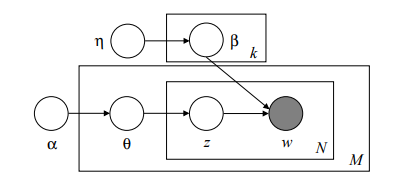
\includegraphics[width=10cm]{images/LDA.png}}	
	\captionof{figure}{\textit{Graphical} Model pada \textit{Smoothed} LDA}
\end{minipage}
\end{adjustbox}

Gambar di atas merupakan model\textit{ smoothed} LDA. Dengan kotak 
pada bagian luar merepresentasikan dokumen, dan kotak pada bagian dalam 
merepresentasikan pengulangan topik dan kata dalam dokumen. Berikut 
penjelasan simbol di atas \label{14}:
\begin{enumerate}[leftmargin=*]
	\item $ \alpha $: parameter \textit{dirichlet prior }distribusi topik terhadap dokumen.
	\item $ \eta $: parameter \textit{dirichlet prior }distribusi kata terhadap topik.
	\item $ \theta $: distribusi topik terhadap dokumen.
	\item $\beta$: distribusi kata terhadap topik.
	\item Z: identitas topik untuk seluruh kata dalam seluruh dokumen
	\item W: identitas seluruh kata dalam seluruh dokumen
	\item K: jumlah topik
	\item M: jumlah dokumen
	\item N: jumlah kata pada dokumen
\end{enumerate}
Berikut ini adalah proses dalam melakukan training LDA topic modelling:
\begin{enumerate}[leftmargin=*]
	\item Menentukan jumlah topik yang diinginkan (K), parameter $ \alpha $, parameter $ \eta $.
	\item Memberikan topik terhadap setiap kata secara acak untuk sementara.
	\item Menghitung nilai probabilitas \textit{topic-word }dan \textit{document-topic}
	\item Mengalikan hasil\textit{ topic-word }dan \textit{document-topic }(Z).
	\item Melakukan random antara 0-1, dan membandingkannya dengan hasil pada tahap 4. Hasil tersebut akan digunakan untuk memberi nilai topik kembali pada setiap kata. Proses ini diulang sampai memenuhi jumlah iterasi.
\end{enumerate}

\subsubsection{\textit{Interjection}}
Fitur \textit{Interjection }adalah fitur untuk menghitung jumlah kata 
\textit{interjection }yang terdapat pada sebuah teks. Contoh kata 
\textit{interjection} adalah "aha", "bah", "wew", "wow", 
"yay", "nah", "uh", dan lain-lain. Fitur ini digunakan untuk 
membantu dalam klasifikasi teks sarkasme, Karena dari 100 data sarkasme 
ditemukan 20 teks mengandung kata interjeksi. Ketika sebuah teks 
mengandung kata interjeksi, teks tersebut cenderung dianggap teks 
sarkasme \cite{5}.
\subsubsection{\textit{Question Word}}
Fitur \textit{Question Word }adalah fitur untuk memberikan nilai 
\textit{true }atau \textit{false}, jika pada teks terdapat kata 
tanya seperti apa, dimana, mengapa, siapa, dan bagaimana. Kata tanya ini 
biasa terdapat pada teks netral, sehingga dapat membantu dalam pemberian 
informasi pada klasifikasi teks netral.
\subsubsection{TF-IDF}
TF-IDF\textit{ }merupakan gabungan dari frekuensi kata (TF) dan 
frekuensi kata pada dokumen (IDF)\textit{.} \textit{Term Frequency} 
(TF) merupakan metode penghitungan jumlah kemunculan kata pada dokumen 
dibagi jumlah kata pada dokumen. TF memiliki persamaan sebagai berikut 
\cite{15}:

\begin{table}[H]
	\small
	\begin{adjustbox}{width=1\textwidth}
	\begin{tabular}{|p{13.55cm}|}
		\hline
		\begin{equation} \label{eqn:TF}
				\textrm{TF}=\frac{\textrm{frekuensi kemunculan kata pada dokumen}}{\textrm{jumlah kata pada dokumen}}
		\end{equation}\\
		\hline
	\end{tabular}
	\end{adjustbox}
\end{table}
\noindent IDF memiliki persamaan sebagai berikut:	
\begin{table}[H]
	\small
	\begin{adjustbox}{width=1\textwidth}
	\begin{tabular}{|p{13.55cm}|}
		\hline
		\begin{equation} \label{eqn:IDF}
		\textrm{IDF}=log\frac{\textrm{jumlah dokumen}}{\textrm{jumlah dokumen yang mengandung kata tertentu}}
		\end{equation}\\
		\hline
	\end{tabular}
	\end{adjustbox}
\end{table}
\noindent TF-IDF memiliki persamaan sebagai berikut:
\begin{table}[H]
	\small
	\begin{adjustbox}{width=1\textwidth}
	\begin{tabular}{|p{13.55cm}|}
		\hline
		\begin{equation} \label{eqn:TF-IDF}
		\textrm{TF-IDF}=\textrm{TF}*\textrm{IDF}
		\end{equation}\\
		\hline
	\end{tabular}
	\end{adjustbox}
\end{table}	
\noindent Ciri-ciri hasil TF-IDF sebagai berikut:
\begin{enumerate}[leftmargin=*]
	\item Bobot akan tinggi jika intensitas kemunculan kata rendah pada banyak dokumen dan intensitas kemunculan kata tinggi pada sebuah dokumen.
	\item Bobot akan rendah jika intensitas kemunculan kata tinggi pada banyak dokumen dan intensitas kemunculan kata rendah pada sebuah dokumen
	\item Bobot akan sangat rendah jika kemunculan suatu kata terdapat pada setiap dokumen.
\end{enumerate}
	
\subsection{Definisi Support Vector Machine (SVM)}
Ide di balik SVM adalah membangun \textit{hyperplane} yang optimal 
agar dapat digunakan dalam klasifikasi pola yang dapat dipisahkan secara 
linear. \textit{Hyperplane} yang optimal adalah \textit{hyperplane} 
yang dipilih dari satu himpunan \textit{hyperplane} yang memaksimalkan 
\textit{margin} pada \textit{hyperplane}. \textit{Margin }adalah 
jarak dari bidang \textit{hyper} ke titik terdekat dari pola. SVM 
dibuat khusus untuk memaksimalkan \textit{margin}, yang akan menjamin 
bahwa pola masukan akan diklasifikasikan dengan benar. SVM biasanya 
digunakan untuk mengklasifikasikan pola. Pola tersebut bisa linear atau 
non-linear \cite{7}. 
\subsubsection{\textit{Support Vector Machine} (SVM)}
Konsep dasar dari \textit{Support Vector Machine }(SVM)\textit{ }
adalah membangun \textit{hyperplane} untuk memisahkan 2 kelas, yaitu 
kelas positif dan kelas negatif dan memaksimalkan \textit{margin}. 
\textit{Margin }adalah jarak antara \textit{hyperplane }dan titik 
data terdekat. Titik data yang terdekat yang menyentuh \textit{
	hyperplane }disebut \textit{Support Vector}. Pada gambar 2.2 
terdapat 6 \textit{support vector}, 3 \textit{support vector }dari 
kelas +1, dan 3 \textit{support vector }dari kelas -1 \cite{16}.

\begin{adjustbox}{width=1\textwidth}
\noindent\begin{minipage}{\linewidth}
	\framebox[\textwidth]{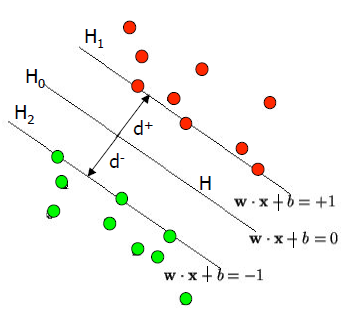
\includegraphics[width=10cm,height=7cm]{images/Hyperplane_SVM.png}}
	\captionof{figure}{\textit{Hyperplane} pada SVM}
\end{minipage}
\end{adjustbox}

Garis lurus di tengah pada gambar 2.2 adalah \textit{hyperplane}. 
Untuk memisahkan 2 kelas pada \textit{Support Vector Machine} 
dibutuhkan \textit{hyperplane }yang optimal. Optimasi bidang \textit{
	hyperplane }dapat diselesaikan dengan teknik optimasi, yaitu \textit{
	Lagrangian Multiplier}. Persamaan pada \textit{hyperplane }dapat 
didefinisikan sebagai berikut \cite{16}:
\begin{table}[H]
	\small
	\begin{adjustbox}{width=1\textwidth}
	\begin{tabular}{|p{13.55cm}|}
		\hline
		\begin{equation}
		w^T.x+b=0
		\end{equation}
		\begin{equation}
		w^T.x+b\geq+1,\textrm{dimana}\ y_i=+1
		\end{equation}
		\begin{equation}
		w^T.x+b \leq -1,\textrm{dimana}\ y_i=-1
		\end{equation}\\
		\hline
	\end{tabular}
	\end{adjustbox}
\end{table}
\vspace{-0.5cm}	
\begin{table}[H]
	\centering
	\begin{tabular}{ll}
		Dimana & :\\
		$X_i$ &: Vektor masukan\\
		$y_i$ &: Kelas\\
		$w^T$ &: Vektor \textit{weight}\\
		$b$ &: Bias
	\end{tabular}
\end{table}
\vspace{-0.8cm}
\noindent Persamaan kernel pada Support Vector Machine sebagai berikut:

\begin{table}[H]
	\caption{Tabel persamaan kernel pada SVM}
	\centering
	\small
	\begin{adjustbox}{width=1\textwidth}
	\begin{tabular}{|p{4.55cm}|p{8.55cm}|}
		\hline
		\textbf{Kernel} & \textbf{Persamaan}\\
		\hline
		
		\begin{center}
			Linear
		\end{center} &
		\vspace{-0.7cm}
		\begin{equation}\label{eqn:kernel-linear}
		K(X_i,X_j)=X_i^T X_j
		\end{equation}\\
		\hline
		
		\begin{center}
			\textit{Polynomial}
		\end{center}&
		\vspace{-0.7cm}
		\begin{equation}
		K(X_i,X_j)=(\gamma X_i^T X_j+\gamma)^4,\gamma>0
		\end{equation}\\
		\hline
		
		\begin{center}
			\textit{Radial Basis Function} (RBF)
		\end{center}&
		\vspace{-0.7cm}
		\begin{equation}
		K(X_i,X_j)=\exp(-\frac{|X_i-X_j|^2}{2\sigma^2})
		\end{equation}\\
		
		\hline
		\textit{\begin{center}
				Sigmoid
			\end{center}}&
			\vspace{-0.7cm}
		\begin{equation}
		K(X_i,X_j)=\tanh(\gamma\ X_i^T X_j+\gamma)
		\end{equation}\\
		\hline
	\end{tabular}
	\end{adjustbox}
\end{table}

\noindent Perhitungan w dapat dilakukan dengan persamaan sebagai berikut:	
\begin{table}[H]
	\small
	\begin{adjustbox}{width=1\textwidth}
	\begin{tabular}{|p{13.55cm}|}
		\hline
		\begin{equation}\label{eqn:weight}
			\textrm{w} = \sum_{i=1}^{m} \alpha_i  y_i x_i
		\end{equation}\\
		\hline
	\end{tabular}
	\end{adjustbox}
\end{table}
\noindent Proses klasifikasi kernel linear dapat dilakukan dengan persamaan:
\begin{table}[H]
	\small
	\begin{adjustbox}{width=1\textwidth}
	\begin{tabular}{|p{13.55cm}|}
		\hline
		\begin{equation}\label{eqn:f(x)}
	f(x)=\sum_{i=1}^{m}\alpha_i y_i K(X_i,X)+b,\ \textrm{m=jumlah data training}
		\end{equation}\\
		\hline
	\end{tabular}
	\end{adjustbox}
\end{table}
Jika nilai $f(x_i )\leq+1$ maka tweet masuk ke kelas positif dan sebaliknya jika $f(x_i )\leq-1$ maka tweet masuk ke kelas negatif. 

\subsubsection{\textit{Multiclass Support Vector Machine}}
Support Vector Machine (SVM) pada awalnya hanya dibuat untuk mengklasifikasikan dua kelas dengan memaksimalkan margin. Pada kenyataanya klasifikasi selalu memiliki lebih dari 2 kelas, sehingga dikembangkan Multiclass SVM agar dapat menangani masalah kelas yang lebih dari 2. Salah satu algoritme untuk klasifikasi multiclass adalah algoritme One versus Rest \cite{17}. 

Prinsip dari One versus Rest adalah membangun kelas sebanyak jumlah klasifikasi kelas. Jika terdapat tiga kelas, maka akan dilakukan perbandingan sebanyak tiga kali. Dan mengambil hasilnya dari nilai keluaran tertinggi. Masalah utama pada klasifikasi ini adalah jumlah data training yang tidak merata \cite{17}. 
\begin{table}[H]
	\caption{Tabel \textit{One versus Rest}}
	\centering
	\small
	\begin{adjustbox}{width=1\textwidth}
	\begin{tabular}{|p{4cm}|p{4cm}|p{4.5cm}|}
		\hline
		\textbf{Y=+1} & \textbf{Y=-1} & \textbf{Hipotesis}\\
		\hline
		Kelas 1 & Bukan kelas 1 &
		$f^1(x)=w^{T1}.x+b^1$\\
		\hline
		Kelas 2 & Bukan kelas 2 &
		$f^2(x)=w^{T2}.x+b^2$\\
		\hline
		Kelas 3 & Bukan kelas 3 &
		$f^3(x)=w^{T3}.x+b^3$\\
		\hline
	\end{tabular}
	\end{adjustbox}
\end{table}
\pagebreak
\subsection{Simplified Sequential Minimal Optimization (SMO)}
\textit{Simplified Sequential Minimal Optimization} (SMO) algoritme adalah teknik optimasi untuk mengatasi dual problem (problem optimization). Algoritme SMO akan dilakukan pengulangan sampai konvergen \cite{18}.
Perhitungan nilai $\alpha$ (alpha) dapat dilakukan dengan persamaan sebagai berikut:

\begin{table}[H]
	\small
	\begin{adjustbox}{width=1\textwidth}
	\begin{tabular}{|p{13.55cm}|}
		\hline
		\begin{equation}
		\textrm{if}\ Y_i \neq Y_j,\ \textrm{L=max}(0,\alpha_j-\alpha_i),\ \textrm{H=min}(C,C+\alpha_j-\alpha_i)
		\end{equation}
		\begin{equation}
		\textrm{if}\ Y_i = Y_j,\ \textrm{L=max}(0,\alpha_j+\alpha_i-C),\ \textrm{H=min}(C,\alpha_j+\alpha_i)
		\end{equation}
		\begin{equation}
		\alpha_j = \alpha_j - \frac{Y_j(E_i-E_j)}{\eta}	
		\end{equation}
		\begin{equation}
		\alpha_i = \alpha_i + Y_i Y_j(\alpha_j(old)-\alpha_i),\ \alpha _{j}= 
		\bigg\{ 
		\begin{gathered}
		H, \textrm{ if } \alpha_{j}>H \\
		\alpha_{j}, \textrm{ if } L\le \alpha _{j}\le H \\
		L, \textrm{ if } \alpha_{j}<L \\
		\end{gathered}
		\end{equation}
		\begin{equation}
		E_k=F(X_k)- Y_k
		\end{equation}
		\begin{equation}
		\eta=2*K(X_i,X_j )-K(X_i,X_i )-K(X_j,X_j)
		\end{equation}\\
		\hline
	\end{tabular}
	\end{adjustbox}
\end{table}

\noindent Perhitungan nilai bias (b) dilakukan dengan persamaan sebagai berikut:
\begin{table}[H]
	\centering
	\small
	\begin{adjustbox}{width=1\textwidth}
	\begin{tabular}{|p{13.55cm}|}
		\hline
		\begin{equation}
		b_1=b-E_i-Y_i (\alpha_i-\alpha_i (old))K(X_i,X_i )-Y_j (\alpha_j-\alpha_j (old))K(X_i,X_j )
		\end{equation}
		\begin{equation}
		b_2=b-E_j-Y_i (\alpha_i-\alpha_i (old))K(X_i,X_j )-Y_j (\alpha_j-\alpha_j (old))K(X_j,X_j )
		\end{equation}
		\begin{equation}
			b= \bigg\{ 
			\begin{gathered}
			b_{1}, \textrm{ if } 0<\alpha _{i}<C \\
			b_{2}, \textrm{ if } 0< \alpha _{j}<C \\
			(b_{1}+b_{2})/2, lainnya \\
			\end{gathered}
		\end{equation}
		\\
		\hline		
	\end{tabular}
	\end{adjustbox}
\end{table}
\pagebreak
\noindent Berikut ini adalah pseudocode Simplified Sequential Minimal Optimization (SMO):

\begin{table}[H]
	\caption{Tabel \textit{Pseudocode} SMO}
	\centering
	\small
	\begin{adjustbox}{width=1\textwidth}
	\begin{tabular}{|p{13.55cm}|}
			\hline
			\begin{enumerate}[label={},leftmargin=*,noitemsep]
				\item Input:
				\item C: regularization parameter
				\item tol: numerical tolerance
				\item max passes: max \# of times to iterate over's without changing
				\item (x(1), y(1)), . . . ,(x(m), y(m)): training data
				\item Output:
				\item $\alpha$ : Lagrange multipliers for solution
				\item b : threshold for solution
				\item Initialize $\alpha_{i}$= 0, b = 0.
				\item Initialize passes = 0.
				\item while (passes $<$ max passes)
				\begin{enumerate}[label={}]
					\item num changed alphas = 0.
					\item for i = 1, . . .m,
					\begin{enumerate}[label={}]
						\item Calculate Ei = f(x(i)) - y(i) using (2.21).
						\item if ((y(i)Ei $<$-tol \&\& $\alpha_{i }$$<$ C) $||$ (y(i)Ei $>$ tol \&\& $\alpha_{i }$$>$ 0))
						\begin{enumerate}[label={}]
							\item Select j!=i randomly
							\item Calculate Ej = f(x(j)) - y(j) using (2.16).
							\item Save old $\alpha$'s: $\alpha_{i}$(old) = $\alpha_{i}$,{ }$\alpha_{j}$(old) = $\alpha_{j}$. 
							\item Compute L and H by (2.12) or (2.13).
							\item if (L == H)
							\item \quad continue to next i.
							\item Compute $\eta$ by (2.17).
							\item if ($\eta \geq$ 0)
							\item \quad continue to next i.
							\item Compute and clip new value for $\alpha_{j }$by (2.14).
							\item if ($|\alpha_{j} - \alpha_{j}$(old)$|< 10^{-5}$)
							\item \quad continue to next i.
							\item Determine value for $\alpha_{i }$by (2.15).
							\item Compute b1 and b2 by (2.18) and 2.19).
							\item Compute b by (2.20).
							\item num changed alphas := num changed alphas + 1.
						\end{enumerate}	
						\item end if		
					\end{enumerate}
					\item end for
					\item if (num changed alphas == 0)
					\item \quad passes := passes + 1
					\item else
					\item \quad passes := 0
				\end{enumerate}
				\item end while	
			\end{enumerate}
			\\
			\hline
	\end{tabular}
	\end{adjustbox}
\end{table}


\subsection{Twitter-scraper}
Twitter-scraper adalah sebuah \textit{script} yang digunakan untuk 
mengambil data \textit{tweet} menggunakan \textit{library }
BeautifullSoup4. BeautifulSoup4 adalah \textit{library }untuk 
mengambil data dari sebuah HTML atau XML. Berikut ini adalah \textit{
	script} cara penggunaan Twitter-scraper pada \textit{command prompt}
:
\begin{table}[H]
	\caption{Tabel metode pada \textit{library} Twitter-scraper}
	\centering
	\small
	\begin{adjustbox}{width=1\textwidth}
	\begin{tabular}{|p{0.5cm}|p{6cm}|p{6cm}|}
		\hline
		\textbf{No} & \textbf{\textit{Script}} & \textbf{Keterangan} \\
		\hline
		1 & Twitterscraper dpr\%20lang\%3Aid -l 500 -o dpr-500.json & \textit{Script }ini digunakan untuk megambil data dengan \textit{keyword }
		pencarian DPR, jumlah \textit{tweet} 500, Bahasa Indonesia, dengan 
		keluaran file berupa json. -l adalah \textit{length} atau jumlah dari 
		\textit{tweet} yang ingin diambil. -o adalah \textit{output} atau 
		keluaran berupa nama file yang diinginkan, dengan \textit{extension} 
		json. \\
		\hline
	\end{tabular}
	\end{adjustbox}
\end{table}
\subsection{Natural Language Toolkit (NLTK)}
NLTK adalah \textit{library} python yang digunakan untuk bekerja 
dengan Bahasa Manusia. Hal-hal yang dapat ditangani NLTK, yaitu \textit{
	tokenize},\textit{ tagging}, \textit{parsing}, dan \textit{
	semantic reasoning}. Berikut ini adalah tabel metode pada \textit{
	library} NLTK:
\begin{table}[H]
	\caption{Tabel metode pada \textit{library} NLTK}
	\centering
	\small
	\begin{adjustbox}{width=1\textwidth}
	\begin{tabular}{|p{0.5cm}|p{6cm}|p{6cm}|}
		\hline
		\textbf{No} & \textbf{Metode} & \textbf{Keterangan} \\
		\hline
		1 & word\_tokenize (String) & Metode ini digunakan untuk melakukan 
		tokenisasi pada sebuah teks, sehingga menghasilkan token-token kata. 
		Keluaran dari metode ini adalah array yang berisi token-token kata. \\
		\hline
	\end{tabular}
	\end{adjustbox}
\end{table}
\subsection{Tweet-preprocessor}
\textit{Library} Tweet-preprocessor adalah \textit{library} 
yang digunakan untuk melakukan \textit{preprocessing} pada data 
\textit{tweet}. \textit{Library }ini menyediakan fitur untuk 
melakukan proses \textit{cleaning}, \textit{tokenizing}, dan 
\textit{parsing }pada \textit{tweet}. Berikut ini adalah tabel 
metode pada \textit{library }Tweet-preprocessor:
\begin{table}[H]
	\caption{Tabel metode pada \textit{library} Tweet-preprocessor}
	\centering
	\small
	\begin{adjustbox}{width=1\textwidth}
	\begin{tabular}{|p{0.5cm}|p{6cm}|p{6cm}|}
		\hline
		\textbf{No} & \textbf{Metode} & \textbf{Keterangan} \\
		\hline
		1 & set\_options(OPT) & Metode ini digunakan untuk melakukan konfigurasi 
		pengaturan teks yang akan dihapus. Pengaturan yang tersedia adalah URL, 
		\textit{mention}, \textit{hashtag}, \textit{reserved words}, 
		\textit{emoji}, \textit{smiley}, \textit{number}. \\
		\hline
		2 & clean (String) & Metode ini digunakan untuk menhapus \textit{
			hashtag},\textit{ mentions}, \textit{emojis}, \textit{reserved 
			words} (RT, FAV), \textit{smileys} dan URLs yang terdapat pada teks. 
		Keluaran dari metode ini adalah String. \\
		\hline
		3 & parse(String) & Metode ini digunakan untuk mengambil teks tertentu 
		pada \textit{tweet}, seperti URL, \textit{mention}, \textit{
			hashtag}, \textit{reserved words}, \textit{emoji}, \textit{
			smiley}, \textit{number}. \\
		\hline
		4 & tokenization(String) & Metode ini digunakan untuk mengubah \textit{
			tweet} yang mengandung kata seperti \textit{hashtag} menjadi \textit{
			\$hashtag\$}. Sebagai contoh, \textit{
			hashtag }"\#DPR", akan menjadi "\textit{
			\$HASHTAG\$}" \\
		\hline
	\end{tabular}
	\end{adjustbox}
\end{table}
\subsection{Sastrawi}
\textit{Library} Sastrawi adalah \textit{library} \textit{stemmer} 
yang digunakan untuk mengubah kata-kata pada Bahasa Indonesia menjadi 
kata dasar. Berikut ini adalah tabel metode pada \textit{library} 
Sastrawi:
\begin{small}
	\begin{longtable}{@{\extracolsep{\fill}}|p{0.5cm}|p{6cm}|p{6cm}|@{}}
		\caption{Tabel metode pada \textit{library} Sastrawi}\\
		\hline
		\textbf{No} & \textbf{Metode} & \textbf{Keterangan} \\
		\hline
		\endhead
		1 & StemmerFactory () & Metode ini merupakan \textit{constructor} 
		untuk membuat \textit{class} \textit{stemmer}. \\
		\hline
		2 & create\_stemmer () & Metode ini untuk menginisialisasi \textit{
			stemmer} yang akan digunakan untuk melakukan \textit{stemming}. \\
		\hline
		3 & stem (String) & Metode ini digunakan untuk melakukan pengubahan 
		kata-kata pada sebuah string berupa teks menjadi kata dasar. Keluaran 
		dari metode ini adalah String, yaitu kalimat yang sudah diubah menjadi 
		kata dasar. \\
		\hline
	\end{longtable}
\end{small}
	
\subsection{IPosTagger}
\textit{Library} IPosTagger adalah \textit{library} yang digunakan 
untuk memberikan \textit{tagging} terhadap kata-kata pada sebuah 
kalimat. Berikut ini adalah metode pada \textit{library} IPosTagger:
\begin{table}[H]
	\caption{Tabel metode pada \textit{library} IPosTagger}
	\centering
	\small
	\begin{adjustbox}{width=1\textwidth}
	\begin{tabular}{|p{0.5cm}|p{6cm}|p{6cm}|}
		\hline
		\textbf{No} & \textbf{Metode} & \textbf{Keterangan} \\
		\hline
		1 & MainTagger (String, String, int, int, int, int, int, boolean, float, 
		int, float, int) & Metode ini merupakan \textit{constructor} untuk 
		membuat \textit{class} \textit{tagger}. Parameter masukan yang 
		diperlukan adalah \textit{file} \textit{lexicon}, \textit{file} 
		\textit{n-gram}, tipe \textit{n-gram}, \textit{maxAffixLength}, 
		\textit{threshold}, \textit{minWordFreq}, \textit{modeAffixTree}
		, \textit{lambdaBigram}, \textit{TwoPhaseType}, \textit{
			BeamFactor}, \textit{UseLexicon}. \\
		\hline
		2 & taggingStr (String) & Metode ini digunakan untuk memberi \textit{
			tagging }pada setiap kata dalam teks. Keluaran dari metode ini adalah 
		array yang berisi kata-kata yang sudah diberi \textit{tag}. \\
		\hline
	\end{tabular}
	\end{adjustbox}
\end{table}
\subsection{Gensim}
Gensim adalah \textit{library open-source} yang menyediakan \textit{
	toolkit }pemodelan topik yang diimplementasikan dengan Python. Berikut 
ini adalah tabel metode pada \textit{library} Gensim: 
\begin{table}[H]
	\caption{Tabel metode pada \textit{library} Gensim}
	\centering
	\small
	\begin{adjustbox}{width=1\textwidth}
	\begin{tabular}{|p{0.5cm}|p{6cm}|p{6cm}|}
		\hline
		\textbf{No} & \textbf{Metode} & \textbf{Keterangan} \\
		\hline
		1 & LdaModel (Array [] [], Array [] [], int, String) & 
		Metode ini merupakan \textit{constructor} yang akan menginisialisasi 
		array[][] \textit{corpus} yang berisi \textit{id} kata dan 
		kemunculan kata, array[][] kamus yang berisi kata dan \textit{
			id} kata, jumlah topik, dan nilai alpha. \\
		\hline
		2 & dictionary (Array []) & Metode ini akan membentuk sebuah kata 
		yang \textit{unique} dengan \textit{id} kata tersebut berdasarkan 
		kata-kata dari data dokumen \textit{training}. \\
		\hline
		3 & doc2bow (String) & Metode ini akan menghitung kemunculan kata dengan 
		\textit{id} katanya. \\
		\hline
		4 & Models.Save (String) & Metode ini untuk menyimpan hasil dari 
		\textit{model} \textit{training} yang ke dalam \textit{file}. \\
		\hline
		5 & Corpora.save (String) & Metode ini untuk menyimpan hasil dari kata 
		\textit{unique} dan \textit{id }kata dari data \textit{training }
		ke dalam \textit{file}. \\
		\hline
		6 & Models.load (String) & Metode ini untuk mengambil kembali \textit{
			model} yang telah disimpan pada sebuah \textit{file }dengan menerima 
		masukan nama \textit{file}. \\
		\hline
		7 & Corpora.load (String) & Metode ini untuk mengambil kembali data yang 
		telah disimpan pada sebuah \textit{file }dengan menerima masukan nama 
		\textit{file}. \\
		\hline
	\end{tabular}
	\end{adjustbox}
\end{table}
\subsection{NumPy}
NumPy adalah \textit{library} yang digunakan untuk perhitungan 
\textit{scientific} pada Python. NumPy memiliki fitur seperti, 
pembuatan array\textit{ }object. Berikut ini adalah tabel metode pada 
\textit{library }NumPy:
\begin{table}[H]
	\caption{Tabel metode pada \textit{library} NumPy}
	\centering
	\small
	\begin{adjustbox}{width=1\textwidth}
	\begin{tabular}{|p{0.5cm}|p{6cm}|p{6cm}|}
		\hline
		\textbf{No} & \textbf{Metode} & \textbf{Keterangan} \\
		\hline
		1 & array (Array) & Metode ini mengubah array \textit{default }dari 
		Python masukan menjadi array numpy atau disebut \textit{nd}array. \\
		\hline
		2 & dot (ndarray, ndarray) & Metode ini digunakan untuk mengalikan nilai 
		dari 2 \textit{nd}array. \\
		\hline
		3 & mean (ndarray) & Metode ini digunakan untuk mendapatkan nilai 
		rata-rata dari sebuah array yang berisi nilai angka. \\
		\hline
		4 & save (String) & Menyimpan nilai dari \textit{nd}array\textit{ }
		ke dalam sebuah \textit{file}. Metode ini menerima masukan berupa 
		nama \textit{file}. \\
		\hline
		5 & load (String) & Mengambil kembali data yang telah disimpan di dalam 
		sebuah \textit{file}. Metode ini menerima masukan berupa nama 
		\textit{file} yang ingin diambil datanya. \\
		\hline
	\end{tabular}
	\end{adjustbox}
\end{table}
\subsection{Scikit-learn}
\textit{Library} \textit{Scikit-learn} merupakan \textit{tools} 
yang digunakan untuk \textit{data mining} dan data \textit{analysis}
. Berikut ini adalah tabel metode pada \textit{library} \textit{
	Scikit-learn}:
%\begin{table}[H]
%	\caption{Tabel metode pada \textit{library} Scikit-learn}
%	\centering

\begin{small}
	\begin{longtable}{@{\extracolsep{\fill}}|p{0.5cm}|p{6cm}|p{6cm}|@{}}
		\caption{Tabel metode pada \textit{library} Scikit-learn}\\
		\hline
		\textbf{No} & \textbf{Metode} & \textbf{Keterangan} \\
		\hline
		\endhead
		1 & shuffle (array [], array []) & Metode ini digunakan untuk 
		melakukan \textit{random }data yang akan digunakan untuk data\textit{ 
			training }dan \textit{testing}. \\
		\hline
		2 & DictVectorizer () & Metode ini merupakan \textit{constructor} yang 
		akan digunakan untuk memetakan nilai fitur menjadi vector. \\
		\hline
		3 & Fit\_transform (array [], array []) & Metode ini digunakan 
		untuk memetakan array dari nilai fitur menjadi vektor berdasarkan fitur 
		pada data \textit{training}. \\
		\hline
		4 & Transform (array [], array []) & Metode ini digunakan untuk 
		memetakan array dari nilai fitur menjadi vektor berdasarkan fitur pada 
		data \textit{testing}, dengan fitur yang tidak terdapat saat 
		melakukan fit\_transform() akan diabaikan. \\
		\hline
		5 & load (String) & Mengambil kembali data yang telah disimpan di dalam 
		sebuah \textit{file}. Metode ini menerima masukan berupa nama 
		\textit{file} yang ingin diambil datanya. \\
		\hline
	\end{longtable}
\end{small}

%\end{table}
\subsection{Bottle}
Bottle adalah sebuah \textit{mini web-framework} pada Python. Bottle 
menyediakan fitur-fitur standar seperti \textit{routing, template, 
	utilities}, dan \textit{server}. Berikut ini adalah metode yang 
digunakan pada sistem analisis sentimen ini:
\begin{table}[H]
	\caption{Tabel metode pada \textit{library} Bottle}
	\centering
	\small
	\begin{adjustbox}{width=1\textwidth}
	\begin{tabular}{|p{0.5cm}|p{6cm}|p{6cm}|}
		\hline
		\textbf{No} & \textbf{Metode} & \textbf{Keterangan} \\
		\hline
		1 & Run() & Metode ini digunakan untuk menjalankan localhost. \\
		\hline
		2 & @route(String) & Metode ini digunakan untuk \textit{routing} web 
		atau mengakses css dan \textit{javascript} \\
		\hline
		3 & @view(String) & Metode ini digunakan untuk menggunakan template view 
		html. \\
		\hline
	\end{tabular}
	\end{adjustbox}
\end{table}
\pagebreak
\section{Tinjauan Studi}
\begin{small}
	\begin{longtable}{@{\extracolsep{\fill}}|p{0.5cm}|p{2cm}|p{2cm}|p{1cm}|p{2cm}|p{3.60cm}|}
		\caption{Tabel Tinjauan Studi}\\
		\hline
		\textbf{No } & \textbf{Peneliti} & \textbf{Judul} & \textbf{Tahun
		} & \textbf{Masalah} & \textbf{Metode/\textit{Accuracy}} \\
		\hline
		\endhead
		1 & Edwin Lunando, Ayu Purwarianti & \textit{Indonesian Social Media 
			Analisis sentimen with Sarcasm Detection } & 2013 & Deteksi teks 
		sarkasme pada analisis sentimen yang masih sulit dilakukan & Pada 
		klasifikasi positif, netral, dan negatif:
		\begin{enumerate}[leftmargin=*]
			\item \textit{Naive Bayes} - 77.40\%
			\item \textit{Maximum Entropy} - 78.40\%
			\item SVM - 77.80\%
		\end{enumerate}
		Pada klasifikasi sarkasme dan non-sarkasme:
		\begin{enumerate}[leftmargin=*]
			\item \textit{Naive Bayes} - 53.10\%
			\item \textit{Maximum Entropy} - 53.80\%
			\item SVM - 54.10\%
		\end{enumerate}\\
		\hline
		2 & Tomas Ptacek, Ivan Habernal, Jun Hong & \textit{Sarcasm Detection 
			on Czech and English }Twitter & 2014 & Deteksi teks sarkasme pada 
		analisis sentimen yang masih sulit dilakukan pada Bahasa Czech Karena 
		banyaknya jenis syntax dan morfologi & Pada klasifikasi sarkasme dan 
		non-sarkasme
		\begin{enumerate}[leftmargin=*]
			\item \textit{Maximum Entropy} - 94.66\%
			\item SVM - 93.13\%
		\end{enumerate}\\
		\hline
		
		3 & Chun-Che Peng, Mohammad Lakis, Jan Wei Pan & \textit{Detecting 
			Sarcasm in Text: An Obvious Solution to a Trivial Problem} & 2015 & 
		Deteksi teks sarkasme pada analisis sentimen yang masih sulit dilakukan 
		& Pada klasifikasi sarkasme dan non-sarkasme:
		\begin{enumerate}
			\item \textit{Naive Bayes} - 62.02\%
			\item \textit{One Class }SVM - 50.00\%
			\item \textit{Gaussian Kernel} - 82.20\% 
		\end{enumerate}
		\\
		\hline
	\end{longtable}		
\end{small}

Pada penelitian satu, Edwin Lunando dan Ayu Purwarianti menggunakan 
fitur \textit{unigram, negativity, number of interjection word, sentiment score} dan 
\textit{question word. }Pada penelitian ini Edwin Lunando dan Ayu 
Purwarianti membuktikan fitur \textit{negativity }dapat meningkatkan 
akurasi dalam menentukan teks sarkasme. Untuk menggunakan fitur \textit{
negativity} akan memakan banyak waktu. Hal ini disebabkan oleh perlunya 
pengetahuan yang cukup mengenai isi dari teks. Hasil klasifikasi dengan 
\textit{direct method} menghasilkan akurasi yang lebih baik dibanding 
\textit{levelled method}. Penelitian ini menggunakan klasifikasi 
\textit{Naive Bayes, Maximum Entropy }dan SVM, dengan akurasi 
tertinggi dihasilkan oleh \textit{Maximum Entropy }\cite{5}.

Pada penelitian dua, Tomas Ptacek, Ivan Habernal dan Jun Hong menggunakan berbagai macam fitur seperti \textit{n-gram}, \textit{pattern}, \textit{part of speech}, \textit{emoticons}, \textit{punctuation based}, \textit{pointedness}, \textit{word-case}. Fitur \textit{pointedness} adalah fitur yang menangani tanda seperti tanda baca tanya (?), tanda baca seru(!) dan \textit{emoticon}. Fitur tersebut tidak digunakan karena penelitian ini tidak menangani \textit{emoticon} pada \textit{tweet}. Fitur \textit{pattern} adalah fitur yang digunakan untuk menghitung kemunculan kata jika memenuhi \textit{threshold} minimal kemunculan kata. Fitur tersebut tidak digunakan, karena penelitian ini sudah menggunakan fitur \textit{unigram} untuk menghitung jumlah kemunculan kata. Pada penelitiannya didapatkan fitur terbaik seperti \textit{n-gram, pointedness, part of speech, emoticon }dan \textit{word-case.} Penelitian ini menggunakan klasifikasi \textit{Maximum Entropy, }dan SVM, dengan akurasi tertinggi dihasilkan oleh \textit{Maximum Entropy} \cite{3}.

Pada penelitian tiga, Chun-Che Peng, Mohammad Lakis, Jan Wei Pan 
menggunakan fitur \textit{n-gram, sentiment score, part of speech, 
capitalization} dan \textit{topic.} Pada penelitian tiga, penggunaan 
fitur \textit{topic} akurasi meningkat secara signifikan. Penelitian 
ini menggunakan klasifikasi \textit{Naive Bayes}, \textit{One Class} SVM, dan \textit{Gaussian Kernel}, dengan akurasi tertinggi 
dihasilkan oleh klasifikasi \textit{Gaussian Kernel }\cite{4}.
\section{Objek Penelitian}
Pada bagian ini akan dibahas objek-objek yang terkait dengan analisis 
sentimen.
\subsection{Twitter}
Twitter adalah sebuah \textit{microblogging service }dengan jumlah 
pengguna 41 juta pada juli 2009. \textit{Tweet} pada Twitter memiliki 
beragam topik dengan batas teks mencapai 140 karakter. Berdasarkan 
penelitian yang dilakukan pada juli 2009, Twitter memiliki 41.7 juta 
pengguna, 1.47 juta relasi social, 4262 \textit{trending topic }dan 
106 juta \textit{tweet}. Pada Twitter pengguna dapat melakukan 
\textit{follow} ke pengguna lain, dan pengguna yang di \textit{follow
} tidak perlu melakukan \textit{follow} kembali. Menjadi seorang 
\textit{follower}, pengguna akan menerima semua pesan yang dibuat 
oleh pengguna yang diikuti\textit{. }Twitter memiliki fitur re
\textit{tweet} yang digunakan untuk menyebarkan informasi kepada 
\textit{follower} pengguna. Istilah pada Twitter terus berkembang, 
contoh RT adalah singkatan untuk \textit{retweet}, "@" diikuti oleh 
nama pengguna atau biasa disebut \textit{mention}, dan "\#" diikuti 
oleh sebuah kata yang disebut \textit{hashtag }\cite{19}.
\subsection{Sarkasme}
Ironi adalah sebuah bentuk penyampaian secara tidak langsung untuk 
menyampaikan perasaan. Karakteristik dari ironi adalah pertentangan 
antara makna dari sebuah kalimat dan maksud dari pembicara yang 
sebenarnya. Salah satu bentuk ironi adalah sarkasme. Sarkasme digunakan 
untuk menyampaikan kritik kepada pendengar atau situasi yang disertai 
dengan penghinaan. Sebagai contoh, ada seorang pegawai yang sedang tidur 
siang saat bekerja, kemudian atasannya berkomentar "jangan bekerja 
terlalu keras!". Jika dilihat dari kalimat, kalimat tersebut tidak 
memiliki makna yang negatif, tetapi kalimat tersebut sebenarnya 
digunakan untuk mengkritik pegawainya yang malas \cite{20}.
\newpage